\section{Classificação de Modulações}

\begin{frame}{Classificação Automática de modulações}
    \begin{itemize}
        \item A Modulação, nas transmissões de dados, refere-se ao processo de modificar uma ou mais características de um sinal chamado de portadora para representar informações ou dados. 
        \item A modulação é necessária para transmitir dados por meio de um meio de comunicação, como cabos de cobre, fibras ópticas ou ondas de rádio.
        \item A classificação automática de modulação (\emph{automatic modulation classification} - AMC) é um problema clássico nas comunicações sem fio modernas. Um dos objetivos da AMC é entender e rotular o espectro de rádio em cenários de comunicação não cooperativos, o que facilita a detecção de falhas, monitoramento de interferência de espectro e acesso dinâmico ao espectro.
    \end{itemize}
\end{frame}

\begin{frame}{Dataset}
    O \emph{dataset} inclue efeitos de canal simulados sintéticamente e gravações pelo ar de $24$ tipos de modulação digital e analógica com as seguintes características:
    \begin{itemize}
        \item $26$ níveis de relação sinal ruído (SNR) ($-20$dB a $30$dB com passo de $2$dB);
        \item $2$ milhões de sinais;
        \item $4096$ realizações (frames) para cada par de modulação e SNR (2.555.904 frames no total);
        \item cada frame com $1024$ amostras In Phase e Quadrature (I/Q) ($2 \times 1024$).
    \end{itemize}
    Foram utilizados apenas 7 tipos de modulações com SNR fixada em $-20$dB.
\end{frame}

\begin{frame}{Treinamento da DNN}
    Para o treinamento do modelo foram definidas as seguintes características:
    \begin{itemize}
        \item Tamanho de cada batch de $64$;
        \item Otimizador de Descida de Gradiente Estocástico (SGD);
        \item $70\%$ das amostras para treinamento e $30\%$ para validação;
        \item Taxa de aprendizagem de $0,05$ e momento de $0,9$;
        \item Critério de loss como entropia cruzada de categoria.
    \end{itemize}
\end{frame}

\begin{frame}{Arquitetura do modelo}
O modelo foi criado com a seguinte arquitetura:
\begin{minipage}[t]{0.45\textwidth}
\begin{itemize}
  \item Entrada ($1024 \times 2$);
        \item Bloco repetido $6$ vezes:
        \begin{itemize}
            \item Conv1D ($40 \times 4$);
            \item BatchNorm;
            \item ReLU;
            \item MaxPool ($2$);
        \end{itemize}
        \item Flatten;
        \item Dense($128$);
        \item BatchNorm;
        \item ReLU;
\end{itemize}
\end{minipage}
\hfill
\begin{minipage}[t]{0.45\textwidth}
\begin{itemize}
  \item Dense($128$);
  \item BatchNorm;
  \item ReLU;
  \item Dense($7$);
  \item Softmax;
\end{itemize}
\end{minipage}
\end{frame}


\begin{frame}{Resultados}
    \begin{table}[H]
    \caption{Acurácias obtidas a partir do modelo comprimido para vários valores de tamanho de bits e $\alpha$.}
    \label{tab_acc}
    \centering
    \begin{tabular}{l|lllll}
    \hline
    \textbf{\diagbox{$\alpha$}{bits}} & \textbf{32 bits}  & \textbf{16 bits} & \textbf{8 bits} & \textbf{4 bits} & \textbf{3 bits}\\ \hline
    \textbf{0,00} &	97,06\%	& 96,93\%	& 97,00\% & 84,18\%	& 83,89\%\\
    \textbf{0,25} &	96,13\%	& 96,68\%	& 95,77\% & 92,03\%	& 84,00\%\\
    \textbf{0,50} &	96,70\%	& 96,41\%	& 96,43\% & 84,31\%	& 83,41\%\\
    \textbf{0,75} & 94,46\%	& 95,20\%  & 95,18\% & 90,55\%	& 83,36\%\\\hline
    \end{tabular}
\end{table}
\end{frame}

\begin{frame}{Resultados}
    \begin{table}[H]
    \caption{Valores de esparsidade obtidos a partir do modelo comprimido para vários valores de tamanho de bits e $\alpha$.}
    \label{tab_spa}
    \centering
    \begin{tabular}{l|lllll}
    \hline
    \textbf{\diagbox{$\alpha$}{bits}} & \textbf{32 bits}  & \textbf{16 bits} & \textbf{8 bits} & \textbf{4 bits} & \textbf{3 bits}\\ \hline
    \textbf{0,25} &	42,17\%	& 47,31\%	& 48,11\% & 45,85\%	& 38,50\%\\
    \textbf{0,50} &	66,26\%	& 60,82\%	& 61,28\% & 60,61\%	& 41,60\%\\
    \textbf{0,75} & 74,78\%	& 69,75\%  & 76,11\% & 68,41\%	& 62,44\%\\\hline
    \end{tabular}
\end{table}
\end{frame}

\begin{frame}{Resultados}
    \begin{table}[H]
    \caption{Tamanho do modelo comprimido para vários valores de tamanho de bits e $\alpha$.}
    \label{tab_siz}
    \centering
    \begin{tabular}{l|lllll}
    \hline
    \textbf{\diagbox{$\alpha$}{bits}} & \textbf{32 bits}  & \textbf{16 bits} & \textbf{8 bits} & \textbf{4 bits} & \textbf{3 bits}\\ \hline
    \textbf{0,00} &	3,18Mb	& 1,59Mb	& 0,80Mb & 0,40Mb	& 0,30Mb\\
    \textbf{0,25} &	1,84Mb	& 0,84Mb	& 0,41Mb & 0,26Mb	& 0,18Mb\\
    \textbf{0,50} &	1,08Mb	& 0,62Mb	& 0,31Mb & 0,16Mb	& 0,17Mb\\
    \textbf{0,75} & 0,80Mb	& 0,48Mb  & 0,19Mb & 0,13Mb	& 0,11Mb\\\hline
    \end{tabular}
\end{table}
\end{frame}


\begin{frame}{Resultados}
    \begin{figure}[H]
    \centering
    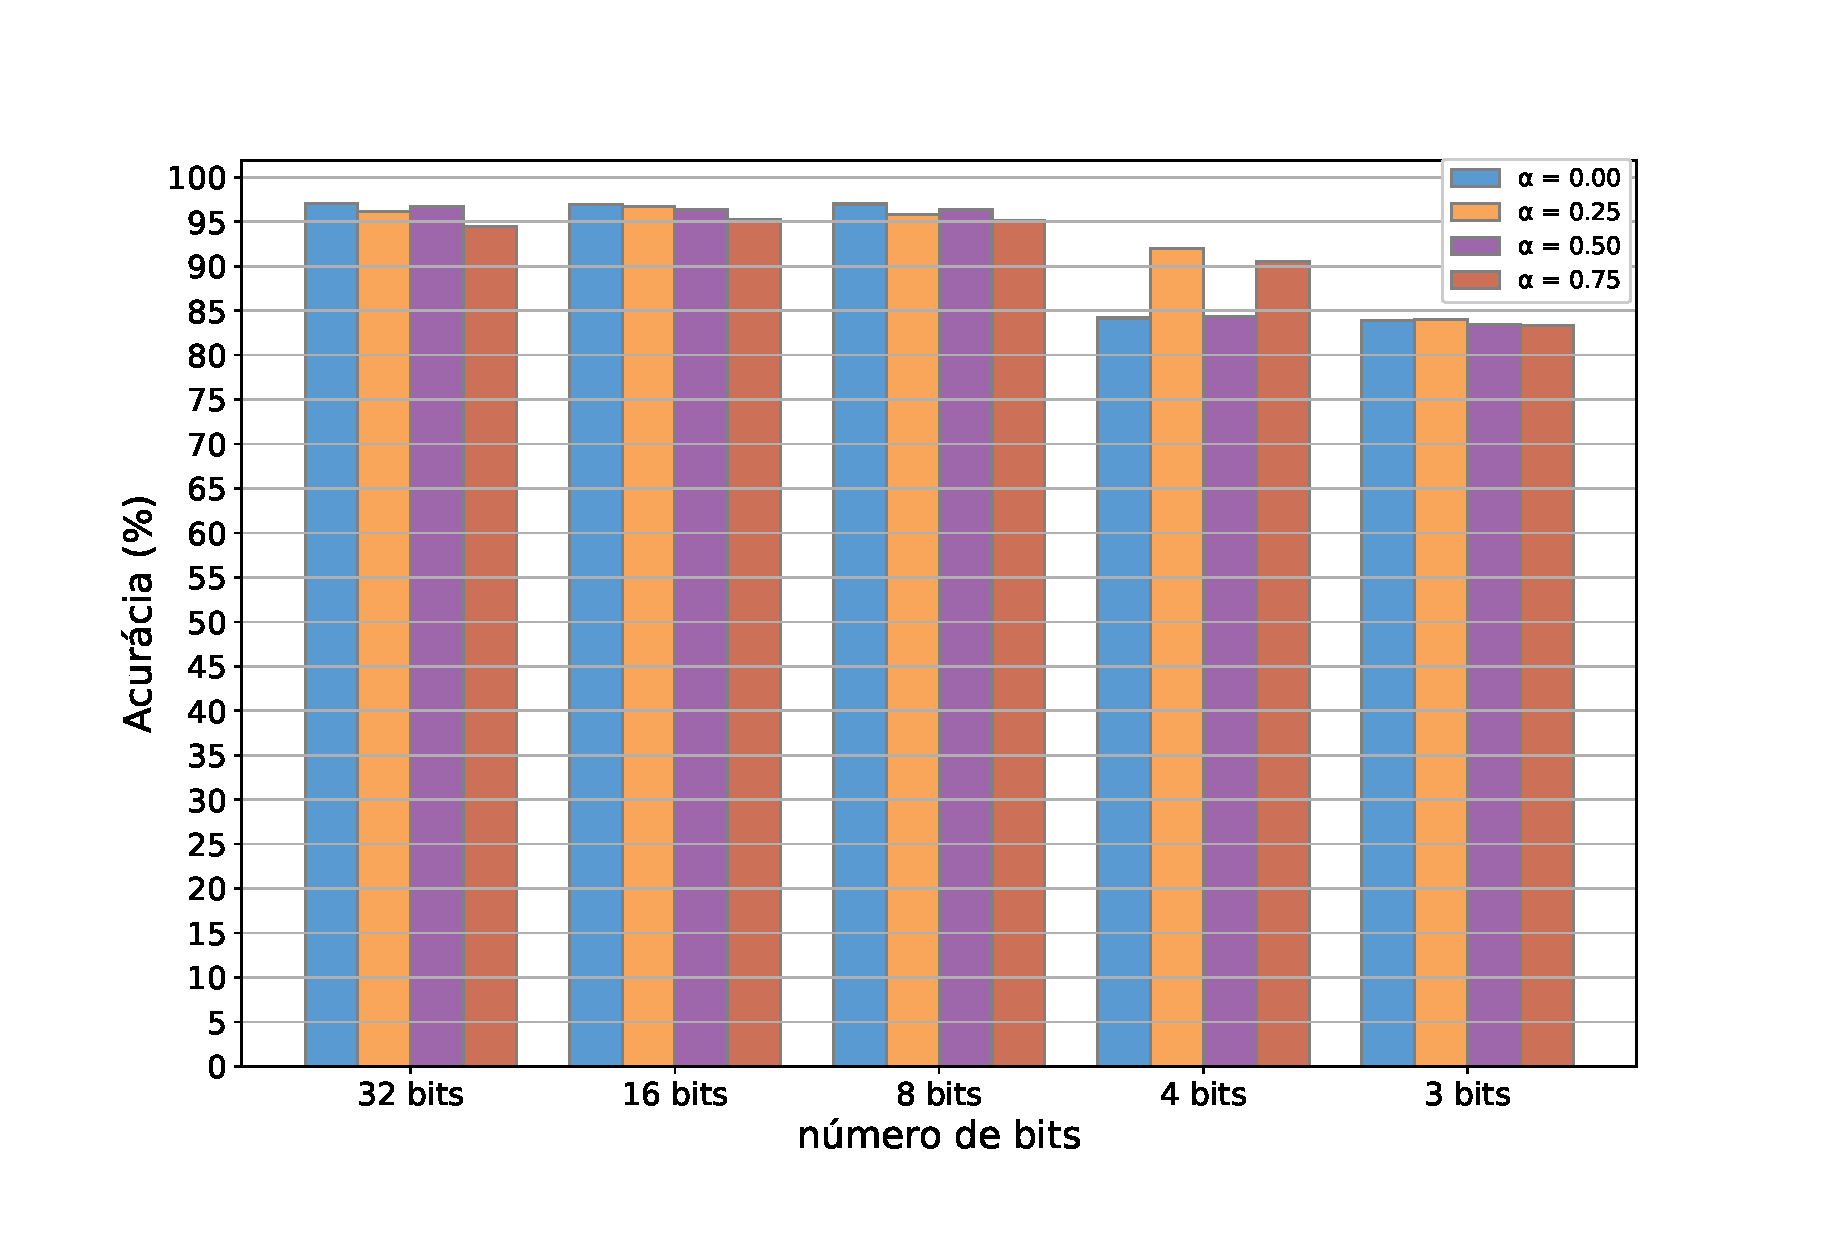
\includegraphics[width=0.7\textwidth]{figuras/accuracies.eps}
    \caption{Acurácias obtidas para diversas configuração de $\alpha$ e número de bits}
    \end{figure}
\end{frame}

\begin{frame}{Resultados}
    \begin{figure}[H]
    \centering
    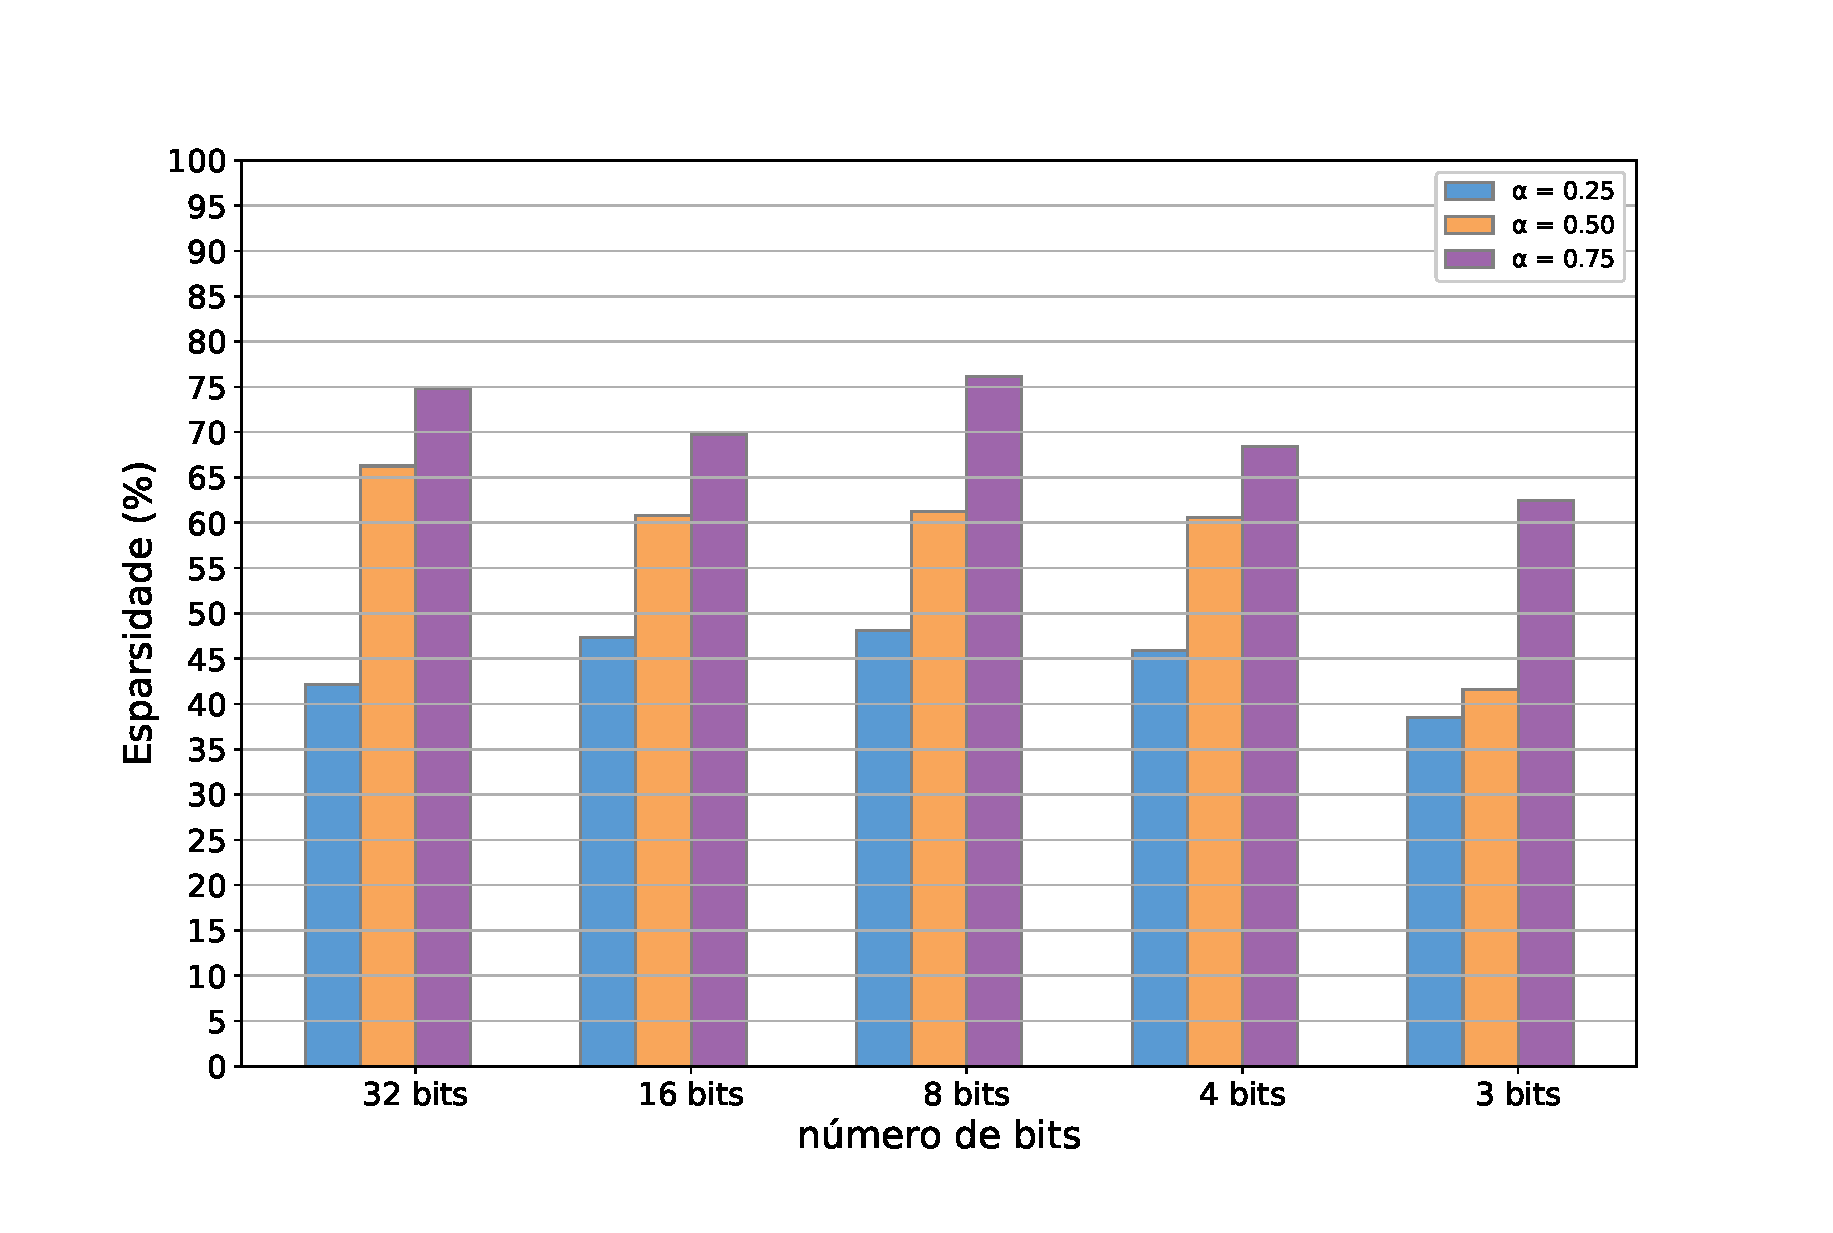
\includegraphics[width=0.7\textwidth]{figuras/sparsity.eps}
    \caption{Esparsidades obtidas para diversas configuração de $\alpha$ e número de bits}
    \end{figure}
\end{frame}

\begin{frame}{Resultados}
    \begin{figure}[H]
    \centering
    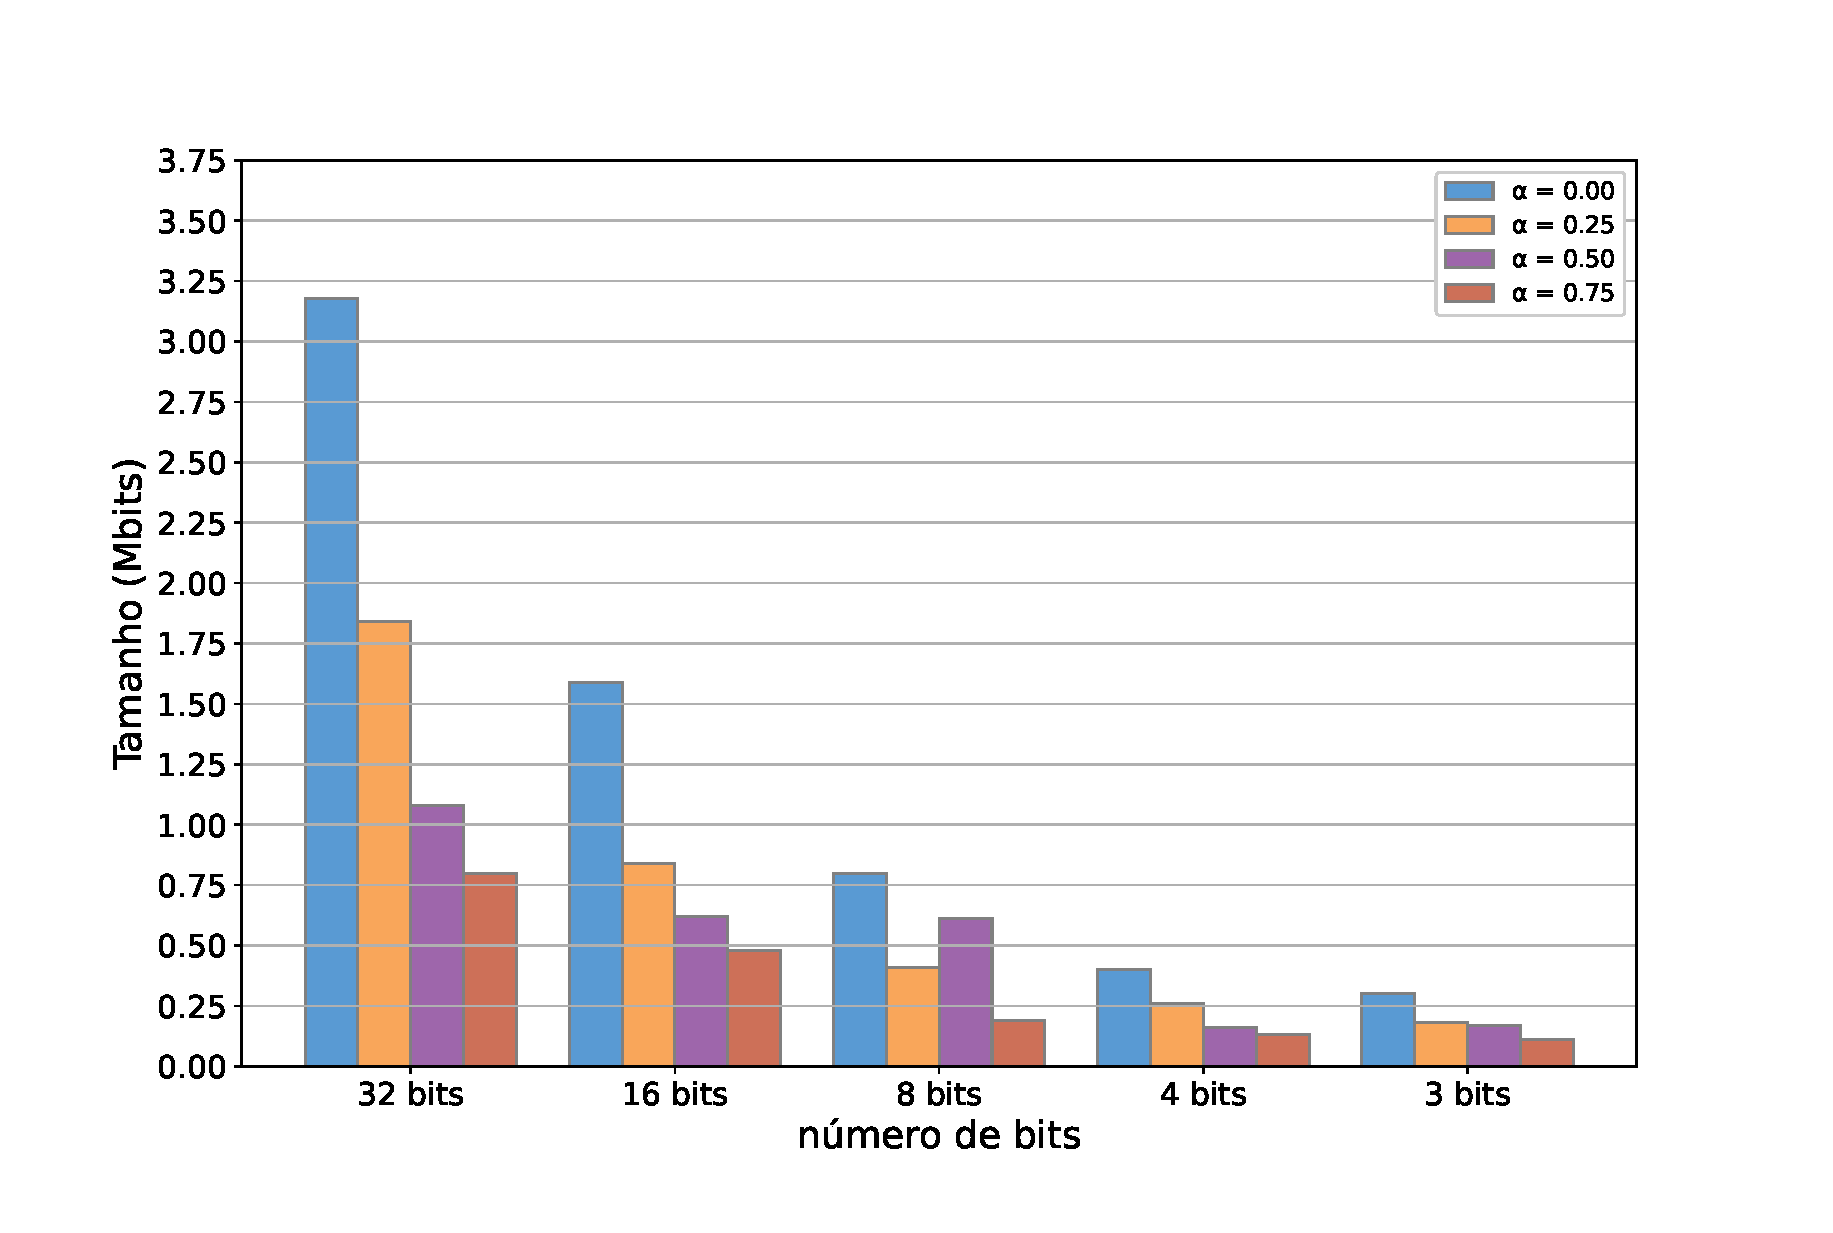
\includegraphics[width=0.7\textwidth]{figuras/sizes.eps}
    \caption{Tamanhos dos modelos obtidos para diversas configuração de $\alpha$ e número de bits}
    \end{figure}
\end{frame}

\begin{frame}{Resultados}
    \begin{figure}[H]
  \centering

  \begin{subfigure}[b]{0.45\textwidth}
    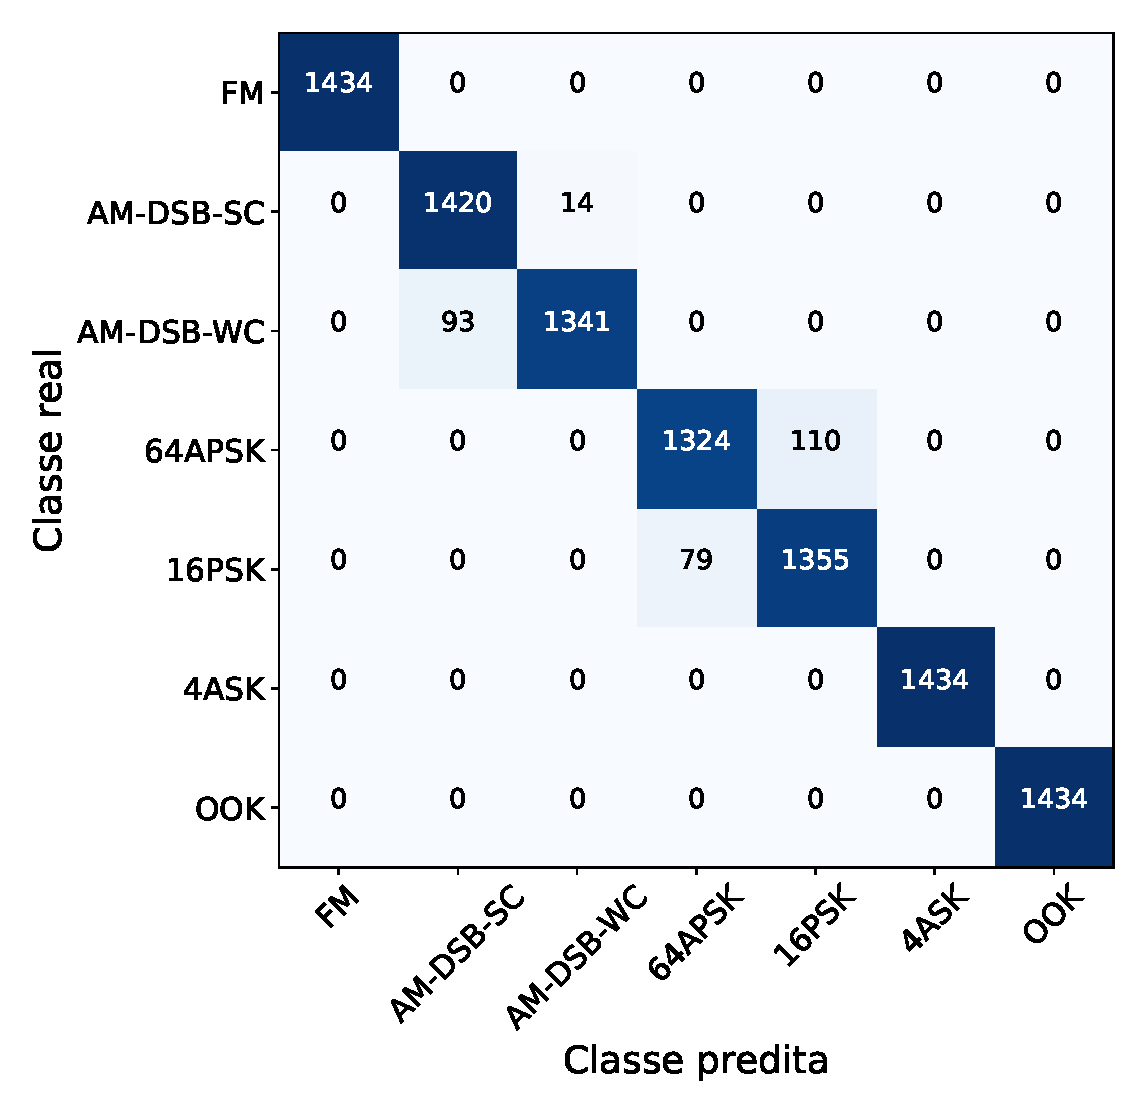
\includegraphics[width=\textwidth]{figuras/cm_nocompress.eps}
    \caption{Modelo não comprimido}
    \label{fig:subfig1}
  \end{subfigure}
  \hfill
  \begin{subfigure}[b]{0.45\textwidth}
    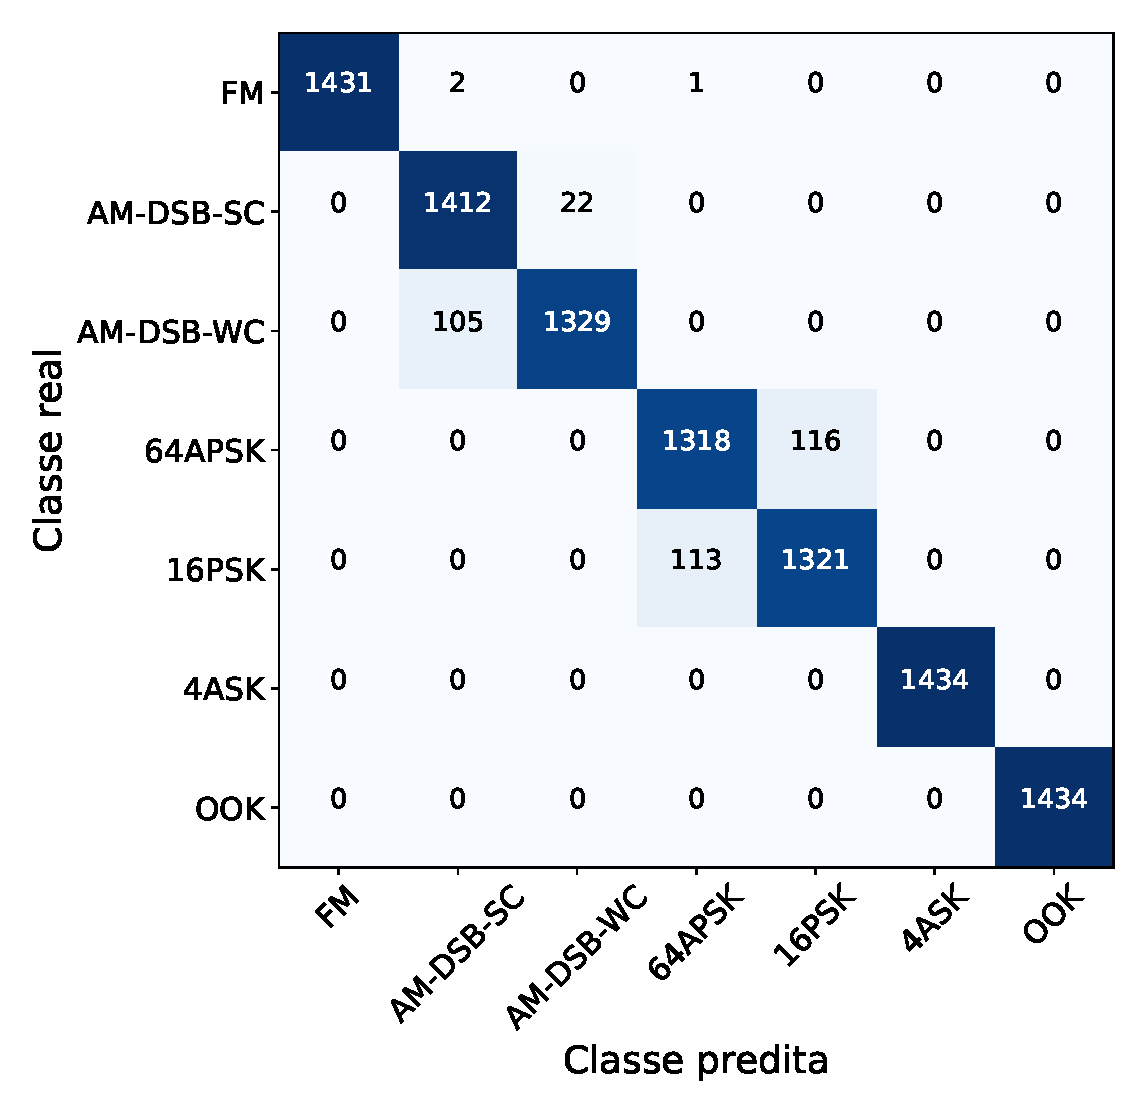
\includegraphics[width=\textwidth]{figuras/cm_8_050.eps}
    \caption{$8$ bits e $\alpha=0,50$}
    \label{fig:subfig2}
  \end{subfigure}
  \caption{Matrizes de confusão de alguns modelos obtidos apos o treinamento}
  \end{figure}

\end{frame}

\begin{frame}{Resultados}
    \begin{figure}[H]
  \centering

  \begin{subfigure}[b]{0.45\textwidth}
    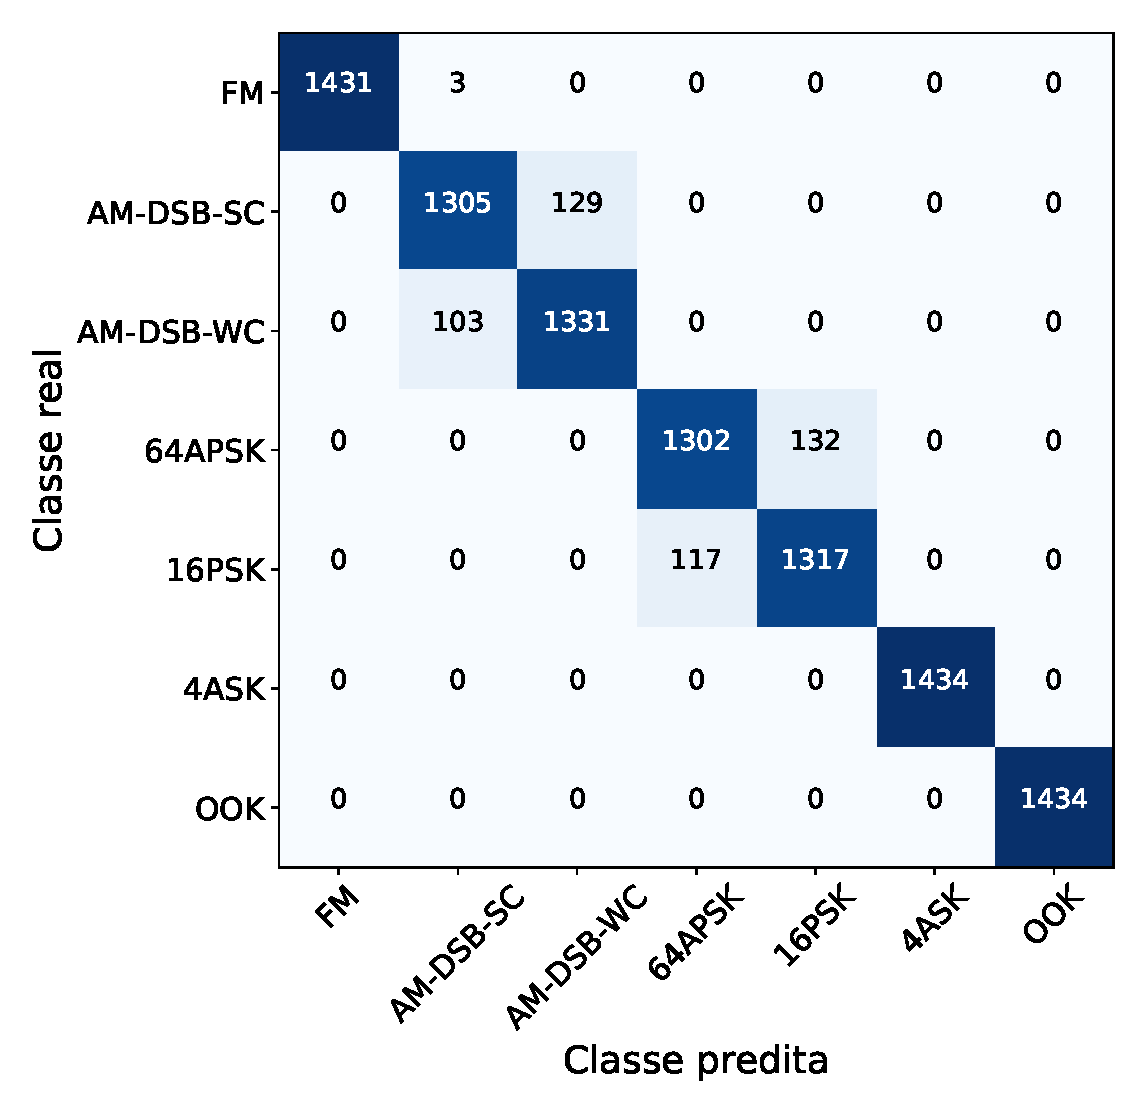
\includegraphics[width=\textwidth]{figuras/cm_8_075.eps}
    \caption{$8$ bits e $\alpha=0,75$}
    \label{fig:subfig1}
  \end{subfigure}
  \hfill
  \begin{subfigure}[b]{0.45\textwidth}
    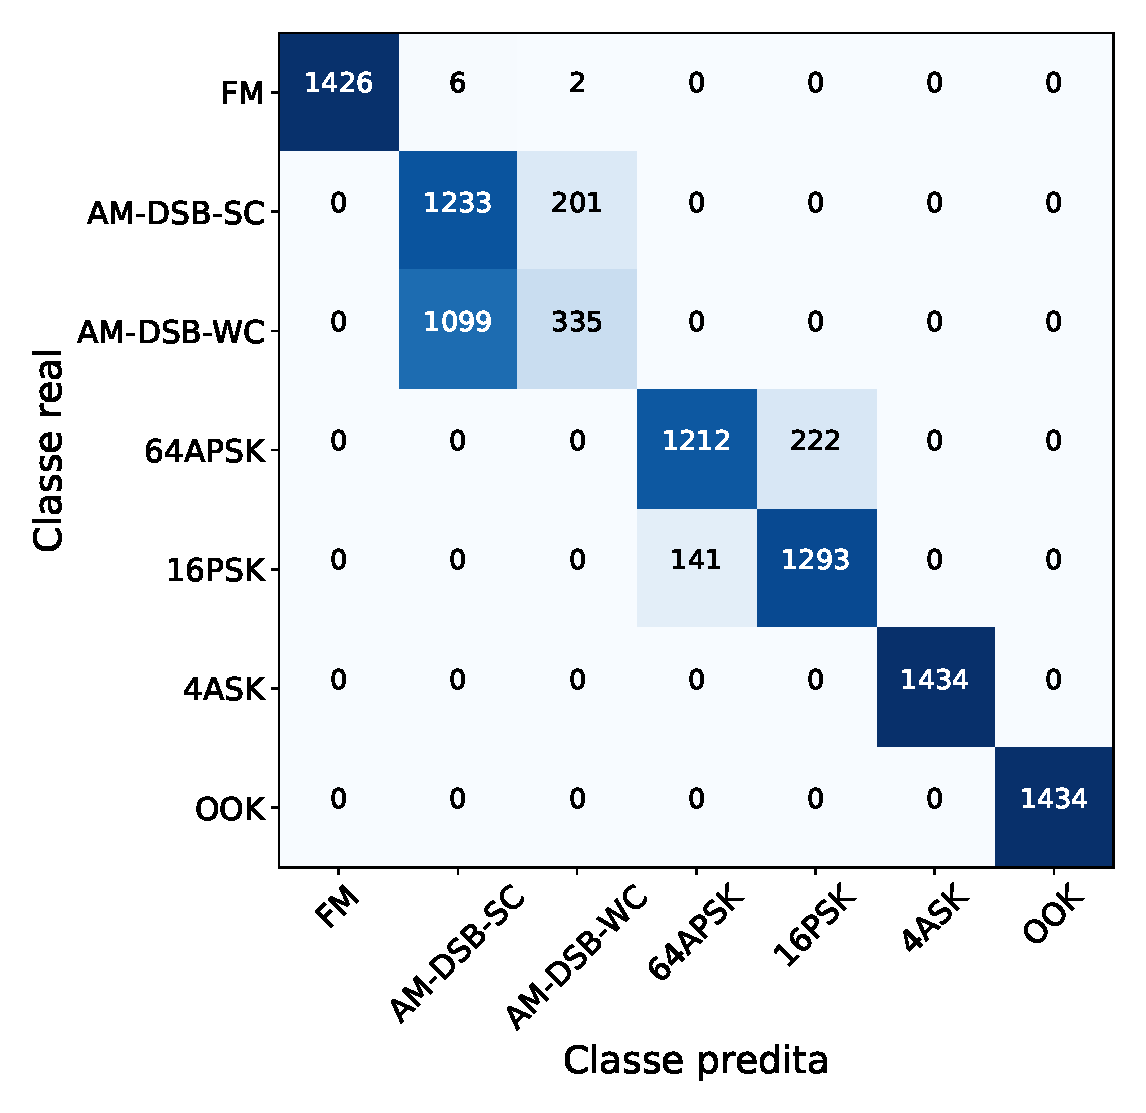
\includegraphics[width=\textwidth]{figuras/cm_3_075.eps}
    \caption{$3$ bits e $\alpha=0,75$}
    \label{fig:subfig2}
  \end{subfigure}
  \caption{Matrizes de confusão de alguns modelos obtidos apos o treinamento}
  \end{figure}

\end{frame}
